
\sektion{Introduction}

\frame{\frametitle{Language fundamentals} 
  \begin{itemize}
    \item Statically typed, \textbf{hybrid} programming language for the JVM
    \item Fully \textbf{interoperable} with Java (1.6)
    \item Runs on \textbf{Android}, compiles to \textbf{JavaScript}
    \item Focuses on \textbf{industry}, tooling and safety
    \item \textbf{Open source} compiler and tools (Apache 2 license)
  \end{itemize}
}

\frame{\frametitle{Historic abstract} 
  \begin{itemize}
    \item Development started 2010
    \item \href{https://blog.jetbrains.com/kotlin/2016/02/kotlin-1-0-released-pragmatic-language-for-jvm-and-android/}{Version 1.0} released February, 2016
    \item Developed by JetBrains (IntelliJ, ReSharper, \ldots)
  \end{itemize}

\vspace{10.0pt}

\begin{figure}[h]
\centering
  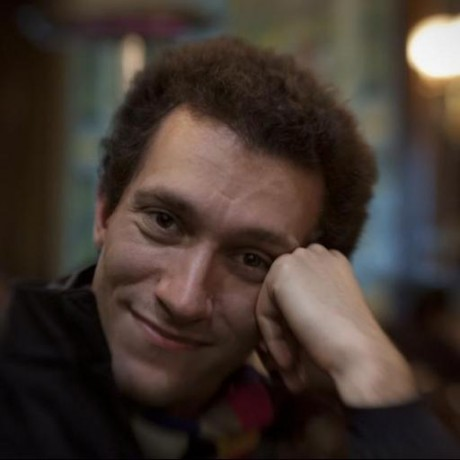
\includegraphics[height=2.0cm]{andrey}
  \vspace{-10.0pt}
  \caption{Andrey Breslav}
\end{figure}
}


\frame{\frametitle{Yet another JVM language?}
\begin{figure}[h]
  \centering
  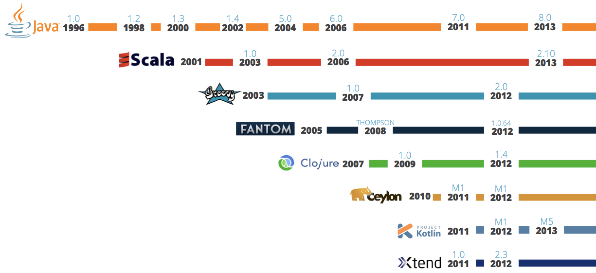
\includegraphics[width=10cm]{jvm_languages}
  \vspace{-10.0pt}
  \caption{Source: \href{https://zeroturnaround.com/rebellabs/the-adventurous-developers-guide-to-jvm-languages-java-scala-groovy-fantom-clojure-ceylon-kotlin-xtend/}{RebelLabs}}
\end{figure}
}

\frame{\frametitle{Java is dead, long live Java}
\quotes{Most people talk about Java the language, and this may sound odd coming from me, but I could hardly care less. \\ At the core of the Java ecosystem is the JVM.}
\textbf{\small{James Gosling,}}\\
\textbf{\tiny{Creator of the Java Programming Language (2011, TheServerSide)}}
}

\fullimage{java_no_cool}

\frame{\frametitle{Yet another JVM language!}
  \begin{itemize}
    \item Nothing new, just the best of all of them
    \item Easy to get started with
    \item Well known company with good tooling support
    \item ``Scala for the \sout{dummies} masses''
  \end{itemize}
}